\documentclass[journal,12pt,twocolumn]{IEEEtran}

\usepackage{setspace}
\usepackage{gensymb}
\singlespacing
\usepackage[cmex10]{amsmath}

\usepackage{amsthm}

\usepackage{mathrsfs}
\usepackage{txfonts}
\usepackage{stfloats}
\usepackage{bm}
\usepackage{cite}
\usepackage{cases}
\usepackage{subfig}

\usepackage{longtable}
\usepackage{multirow}

\usepackage{enumitem}
\usepackage{mathtools}
\usepackage{steinmetz}
\usepackage{tikz}
\usepackage{circuitikz}
\usepackage{verbatim}
\usepackage{tfrupee}
\usepackage[breaklinks=true]{hyperref}
\usepackage{graphicx}
\usepackage{tkz-euclide}

\usetikzlibrary{calc,math}
\usepackage{listings}
    \usepackage{color}                                            %%
    \usepackage{array}                                            %%
    \usepackage{longtable}                                        %%
    \usepackage{calc}                                             %%
    \usepackage{multirow}                                         %%
    \usepackage{hhline}                                           %%
    \usepackage{ifthen}                                           %%
    \usepackage{lscape}     
\usepackage{multicol}
\usepackage{chngcntr}

\DeclareMathOperator*{\Res}{Res}

\renewcommand\thesection{\arabic{section}}
\renewcommand\thesubsection{\thesection.\arabic{subsection}}
\renewcommand\thesubsubsection{\thesubsection.\arabic{subsubsection}}

\renewcommand\thesectiondis{\arabic{section}}
\renewcommand\thesubsectiondis{\thesectiondis.\arabic{subsection}}
\renewcommand\thesubsubsectiondis{\thesubsectiondis.\arabic{subsubsection}}


\hyphenation{op-tical net-works semi-conduc-tor}
\def\inputGnumericTable{}                                 %%

\lstset{
%language=C,
frame=single, 
breaklines=true,
columns=fullflexible
}
\begin{document}

\newcommand{\BEQA}{\begin{eqnarray}}
\newcommand{\EEQA}{\end{eqnarray}}
\newcommand{\define}{\stackrel{\triangle}{=}}
\bibliographystyle{IEEEtran}
\raggedbottom
\setlength{\parindent}{0pt}
\providecommand{\mbf}{\mathbf}
\providecommand{\pr}[1]{\ensuremath{\Pr\left(#1\right)}}
\providecommand{\qfunc}[1]{\ensuremath{Q\left(#1\right)}}
\providecommand{\sbrak}[1]{\ensuremath{{}\left[#1\right]}}
\providecommand{\lsbrak}[1]{\ensuremath{{}\left[#1\right.}}
\providecommand{\rsbrak}[1]{\ensuremath{{}\left.#1\right]}}
\providecommand{\brak}[1]{\ensuremath{\left(#1\right)}}
\providecommand{\lbrak}[1]{\ensuremath{\left(#1\right.}}
\providecommand{\rbrak}[1]{\ensuremath{\left.#1\right)}}
\providecommand{\cbrak}[1]{\ensuremath{\left\{#1\right\}}}
\providecommand{\lcbrak}[1]{\ensuremath{\left\{#1\right.}}
\providecommand{\rcbrak}[1]{\ensuremath{\left.#1\right\}}}
\theoremstyle{remark}
\newtheorem{rem}{Remark}
\newcommand{\sgn}{\mathop{\mathrm{sgn}}}
\providecommand{\abs}[1]{\vert#1\vert}
\providecommand{\res}[1]{\Res\displaylimits_{#1}} 
\providecommand{\norm}[1]{\lVert#1\rVert}
%\providecommand{\norm}[1]{\lVert#1\rVert}
\providecommand{\mtx}[1]{\mathbf{#1}}
\providecommand{\mean}[1]{E[ #1 ]}
\providecommand{\fourier}{\overset{\mathcal{F}}{ \rightleftharpoons}}
%\providecommand{\hilbert}{\overset{\mathcal{H}}{ \rightleftharpoons}}
\providecommand{\system}{\overset{\mathcal{H}}{ \longleftrightarrow}}
	%\newcommand{\solution}[2]{\textbf{Solution:}{#1}}
\newcommand{\solution}{\noindent \textbf{Solution: }}
\newcommand{\cosec}{\,\text{cosec}\,}
\providecommand{\dec}[2]{\ensuremath{\overset{#1}{\underset{#2}{\gtrless}}}}
\newcommand{\myvec}[1]{\ensuremath{\begin{pmatrix}#1\end{pmatrix}}}
\newcommand{\mydet}[1]{\ensuremath{\begin{vmatrix}#1\end{vmatrix}}}
\numberwithin{equation}{subsection}
\makeatletter
\@addtoreset{figure}{problem}
\makeatother
\let\StandardTheFigure\thefigure
\let\vec\mathbf
\renewcommand{\thefigure}{\theproblem}
\def\putbox#1#2#3{\makebox[0in][l]{\makebox[#1][l]{}\raisebox{\baselineskip}[0in][0in]{\raisebox{#2}[0in][0in]{#3}}}}
     \def\rightbox#1{\makebox[0in][r]{#1}}
     \def\centbox#1{\makebox[0in]{#1}}
     \def\topbox#1{\raisebox{-\baselineskip}[0in][0in]{#1}}
     \def\midbox#1{\raisebox{-0.5\baselineskip}[0in][0in]{#1}}
\vspace{3cm}
\title{Assignment 3}
\author{Vijay Varma - AI20BTECH11012}
\maketitle
\newpage
\bigskip
\renewcommand{\thefigure}{\theenumi}
\renewcommand{\thetable}{\theenumi}
%
Download latex-tikz codes from 
%
\begin{lstlisting}
https://github.com/KBVijayVarma/EE3900/tree/main/Assignment_3
\end{lstlisting}
%
Download python codes from 
%
\begin{lstlisting}
https://github.com/KBVijayVarma/EE3900/tree/main/Assignment_3/codes
\end{lstlisting}
\section*{\textbf{Problem (Construction Q 2.19)}}
Draw a circle of radius 3 and any two of its diameters. Draw the ends of these diameters. What figure do you get?
\section*{\textbf{Solution}}
Let us draw a Circle of radius 3 with centre O.

Let AB and CD be any two diameters of this circle such that $\overline{\rm AB} \not \perp \overline{\rm CD}$. 

A Quadrilateral ACBD is formed by joining the ends of these diameters.

Diameters $\overline{\rm AB}$ and $\overline{\rm CD}$ are of equal length i.e., $\overline{\rm AB} = \overline{\rm CD}$.

Hence diagonals of the Quadrilateral ACBD are of equal length.

Radii of the Circle are of equal length, i.e., $\overline{\rm OA}$ = $\overline{\rm OB}$ = $\overline{\rm OC}$ = $\overline{\rm OD}$ = 3.

\begin{figure}[!h]
\centering
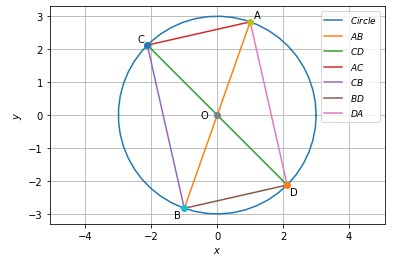
\includegraphics[width=\columnwidth]{fig1.jpg}
\caption{Rectangle}
\label{rectangle}
\end{figure}

$\therefore$ Diagonals $\overline{\rm AB} = \overline{\rm CD}$ and  $\overline{\rm OA} = \overline{\rm OB} = \overline{\rm OC} = \overline{\rm OD}$

So, the Diagonals of the Quadrilateral ACBD, $\overline{\rm AB}$ and $\overline{\rm CD}$ are of equal length and are bisecting each other.

\textbf{Rectangle} is a Quadrilateral having Diagonals of equal length and the Diagonals should bisect each other.

Hence, the Quadrilateral ACBD is a \textbf{Rectangle}. 

This can be verified from above figure \ref{rectangle}. \\

Now, let us take two diameters PQ and RS of the circle such that $\overline{\rm PQ} \perp \overline{\rm RS}$ .

From above, we get that Diagonals $\overline{\rm PQ} = \overline{\rm RS}$ and  $\overline{\rm OP} = \overline{\rm OQ} = \overline{\rm OR} = \overline{\rm OS}$.

But $\overline{\rm PQ} \perp \overline{\rm RS}$ .

So, the Diagonals of the Quadrilateral PRQS, $\overline{\rm PQ}$ and $\overline{\rm RS}$ are of equal length and are bisecting each other perpendicularly.

\textbf{Square} is a Quadrilateral having Diagonals of equal length and the Diagonals should bisect each other perpendicularly.

Hence, the Quadrilateral PRQS is a \textbf{Square}.

\begin{figure}[!h]
\centering
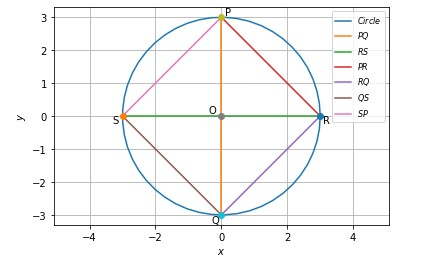
\includegraphics[width=\columnwidth]{fig2.jpg}
\caption{Square}
\label{square}
\end{figure}

This can be verified from above figure \ref{square}.

\textbf{Therefore, the figure is a Rectangle if the Diameters are not perpendicular and is a Square if the Diameters are perpendicular.}


\end{document}